\documentclass[12pt]{book}
\usepackage[brazil]{babel}
\usepackage[utf8]{inputenc}
\usepackage{hyperref}
\usepackage{listings}
\usepackage{longtable}
\usepackage{inconsolata} % fonte monoespaçada bonita

\usepackage{xcolor}
\usepackage{graphicx}
\usepackage{amsmath, amssymb}
\usepackage{geometry}
\geometry{a4paper, margin=2.5cm}

\definecolor{codegray}{rgb}{0.5,0.5,0.5}
\definecolor{codepurple}{rgb}{0.58,0,0.82}
\definecolor{backcolour}{rgb}{0.95,0.95,0.92}

\lstset{
  basicstyle=\ttfamily\footnotesize,
  breaklines=true,
  keywordstyle=\color{blue},
  commentstyle=\color{gray},
  stringstyle=\color{orange},
  showstringspaces=false,
  columns=flexible,
  frame=single,
  backgroundcolor=\color{gray!5}
}

\lstdefinelanguage{JavaScript}{
  keywords={break, case, catch, class, const, continue, debugger, default, delete, do, else, export, extends,
            finally, for, function, if, import, in, instanceof, let, new, return, super, switch, this, throw, try,
            typeof, var, void, while, with, yield},
  keywordstyle=\color{blue}\bfseries,
  ndkeywords={true, false, null, undefined},
  ndkeywordstyle=\color{red}\bfseries,
  identifierstyle=\color{black},
  sensitive=true,
  comment=[l]{//},
  morecomment=[s]{/*}{*/},
  commentstyle=\color{gray}\ttfamily,
  stringstyle=\color{orange},
  morestring=[b]',
  morestring=[b]",
}

% Estilo global para todos os códigos
\lstset{
  language=JavaScript,
  basicstyle=\ttfamily\footnotesize,
  keywordstyle=\color{blue},
  commentstyle=\color{gray},
  stringstyle=\color{orange},
  showstringspaces=false,
  breaklines=true,
  numbers=none,
  backgroundcolor=\color{white}, % <-- fundo branco
  frame=single,
  tabsize=2,
  captionpos=b
}

\title{Desenvolvimento de aplicativos com React Native}
\author{Herbert Rausch}
\date{\today}

\begin{document}

\maketitle
\tableofcontents

\chapter{Introdução ao React com Expo e Docker}

\section{O que é o React?}



O React é uma biblioteca JavaScript para construção de interfaces de usuário. Criado por Jordan Walke no Facebook em 2011, foi tornado open-source em 2013. Desde então, tornou-se amplamente utilizado tanto no desenvolvimento web quanto no mobile, principalmente com o surgimento do React Native.


\section{Por que usar React?}

Entre os principais motivos para utilizar o React estão:

\begin{itemize}
  \item Componentização: permite criar interfaces como blocos reutilizáveis.
  \item Virtual DOM: atualizações eficientes sem recarregar toda a página.
  \item Grande comunidade e ecossistema.
  \item Compatibilidade com frameworks e bibliotecas modernas.
  \item Suporte a múltiplas plataformas com React Native.
\end{itemize}

\section{Tutorial: Criando uma nova Aplicação React com Expo}

Neste tutorial, criaremos um projeto React com o framework Expo, utilizando Docker para isolar o ambiente de desenvolvimento. O Expo é uma ferramenta que facilita o desenvolvimento de aplicativos React Native e também oferece suporte para execução no navegador via `expo start --web` \cite{reactCreatingApp,expoTutorial}.

\subsection{Templates do Expo}

Ao criar um projeto com o Expo usando o comando `expo init`, o usuário pode escolher diferentes templates, conforme descrito na documentação oficial \cite{expoCreateExpo}.

\begin{longtable}{|p{3.5cm}|p{3.5cm}|p{6.5cm}|}
\hline
\textbf{Template} & \textbf{Descrição} & \textbf{Inclui} \\
\hline
blank & Projeto mínimo com JavaScript & React Native sem nenhuma biblioteca adicional \\
\hline
blank (TypeScript) & Igual ao blank, mas com TypeScript & TypeScript + suporte a tipos \\
\hline
tabs (JavaScript) & Projeto com navegação por abas & Navegação, organização de pastas, componentes prontos \\
\hline
tabs (TypeScript) & Mesmo que tabs, com TypeScript & Tabs + TypeScript + organização estruturada \\
\hline
\end{longtable}

Neste projeto, escolhemos o template `blank`.

\subsection{Criação do projeto com Docker}

Utilizamos Docker para criar o projeto React com Expo, garantindo um ambiente consistente entre diferentes sistemas operacionais.

\subsubsection*{Makefile}

\begin{lstlisting}[caption={Comando Make para criar o projeto com Expo}]
IMAGE_NAME=react-app
APP_DIR=app

init:
	mkdir -p $(APP_DIR)
	docker run --rm -it -v "$$(pwd)/$(APP_DIR)":/app -w /app node:18-alpine \
		sh -c "npm install -g expo-cli && \
		       expo init . --template blank --npm --yes && \
		       npx expo install react-dom react-native-web @expo/metro-runtime"

build:
	docker build -t $(IMAGE_NAME) .

start:
	docker run -it --rm -p 8081:8081 -v "$$(pwd)/$(APP_DIR)":/app $(IMAGE_NAME)
\end{lstlisting}

\subsubsection*{Explicação dos comandos Docker}

\begin{itemize}
  \item \texttt{--rm}: remove o container após o uso.
  \item \texttt{-it}: roda o container interativamente.
  \item \texttt{-v "$(pwd)/app":/app}: monta a pasta local `app` no diretório `/app` do container.
  \item \texttt{-w /app}: define o diretório de trabalho no container.
\end{itemize}

\subsubsection*{Dockerfile}

\begin{lstlisting}[caption={Dockerfile}]
FROM node:18-alpine

WORKDIR /app

COPY app/package*.json ./
RUN npm install

COPY app .

EXPOSE 8081

CMD ["npx", "expo", "start", "--web"]
\end{lstlisting}
Fonte: \cite{dockerReact}
\subsection{Rodando a aplicação}

Após a criação e build da imagem, executamos:

\begin{lstlisting}[language=bash]
make init    # Executa uma vez para criar o projeto
make build   # Constrói a imagem Docker
make start   # Inicia o app em http://localhost:8081
\end{lstlisting}

\section{Desenvolvimento no navegador com Snack}

O Expo também oferece uma plataforma chamada \textbf{Snack}, que permite criar, editar e testar aplicações React Native diretamente no navegador, de forma semelhante ao CodePen ou CodeSandbox.

\begin{quote}
Essa solução é oferecida pelo próprio Expo e se chama Snack. O Snack é a solução de desenvolvimento React Native web do Expo. Com ele, conseguimos criar projetos completos e emular seu funcionamento diretamente no navegador. Algo muito parecido com o que temos com outras ferramentas web, tais como: CodePen (https://codepen.io/) e CodeSandBox (https://codesandbox.io/).
\end{quote}

\begin{quote}
Esta solução pode ser acessada diretamente pelo site oficial (https://snack.expo.dev/). O editor é bastante poderoso e oferece recursos avançados. É possível escolher a versão do Expo, conectar os apps com o seu dispositivo (de forma semelhante a que fizemos anteriormente), configurar atalhos e até mesmo mudar o tema para claro ou escuro.
\end{quote}

\section{Arquivos gerados pelo Expo}

Após a criação do projeto, os principais arquivos e pastas gerados são:

\begin{itemize}
  \item \texttt{package.json}: gerencia dependências e scripts.
  \item \texttt{index.js}: é o ponto de entrada principal de uma aplicação React.
  \item \texttt{App.js}: componente principal da aplicação.
  \item \texttt{assets/}: todos os arquivos estáticos da nossa aplicação, como, por exemplo, as imagens. Todas as imagens que vamos utilizar em nosso app deverão ser colocadas nessa pasta. 
  \item \texttt{/node\_modules}, onde estão contidas as dependências do projeto.
\end{itemize}


\subsection*{index.js}
\begin{lstlisting}[language=JavaScript, caption={Conteúdo de index.js}]
import { registerRootComponent } from 'expo';

import App from './App';

// registerRootComponent calls AppRegistry.registerComponent('main', () => App);
// It also ensures that whether you load the app in Expo Go or in a native build,
// the environment is set up appropriately
registerRootComponent(App);

\end{lstlisting}

\subsection*{App.js}


\begin{lstlisting}[language=JavaScript, caption={Novo conteúdo de App.js}]
import React from 'react';
import { View, Text, StyleSheet } from 'react-native';

export default function App() {
  return (
    <View style={styles.container}>
      <Text style={styles.text}>Bem-vindo ao React com Expo!</Text>
    </View>
  );
}

const styles = StyleSheet.create({
  container: {
    flex: 1,
    justifyContent: 'center',
    alignItems: 'center'
  },
  text: {
    fontSize: 20,
    fontWeight: 'bold'
  }
});
\end{lstlisting}

No início do arquivo \texttt{App.js}, encontramos algumas importações essenciais para o funcionamento do React Native. Primeiramente, é importado o \texttt{React} da biblioteca principal, o que permite a utilização de seus recursos de componentização. Em seguida, são importados três elementos da biblioteca \texttt{react-native}: \texttt{StyleSheet}, \texttt{Text} e \texttt{View}. Esses componentes são convertidos em elementos nativos quando a aplicação é executada em diferentes plataformas (Android, iOS ou web). Também é importado o componente \texttt{StatusBar}, disponibilizado pelo Expo, que ajuda no controle visual da barra de status do dispositivo.

Na sequência, é declarada e exportada a função \texttt{App}, que define o componente principal da aplicação. Esse tipo de estrutura é conhecido como \textbf{componente funcional}. Alternativamente, o React também permite a criação de \textbf{componentes baseados em classe}, como veremos em tópicos futuros.

Dentro da função \texttt{App}, utilizamos a sintaxe JSX para definir a interface visual da aplicação. O retorno da função contém uma estrutura com o componente \texttt{<View>} englobando um componente \texttt{<Text>}. No contexto do React Native, o \texttt{<View>} funciona de maneira semelhante à tag \texttt{<div>} do HTML, enquanto o \texttt{<Text>} se comporta como um parágrafo, similar à tag \texttt{<p>}.

Por fim, temos um objeto chamado \texttt{styles}, criado por meio da função \texttt{StyleSheet.create}. Esse objeto define os estilos utilizados na aplicação, de forma semelhante ao CSS tradicional. Utilizar esse padrão permite manter os estilos organizados, reutilizáveis e mais integrados ao ambiente do React Native.

\paragraph{}
É importante destacar que o nome da função exportada no arquivo \texttt{App.js} precisa coincidir com o nome importado no arquivo \texttt{index.js}. No caso dos projetos criados com Expo, o \texttt{index.js} utiliza a função \texttt{registerRootComponent(App)}, assumindo que o componente principal da aplicação está definido e exportado com o nome \texttt{App}. Caso haja divergência de nomes, a aplicação não será inicializada corretamente, pois o componente principal não será localizado pelo sistema.




\section{Como o React funciona: Componentes e Virtual DOM}

\subsection*{A ideia central: tudo é componente}

A principal característica do React é sua abordagem baseada em componentes reutilizáveis. Em vez de escrever todo o código HTML em um único arquivo, como era comum no desenvolvimento tradicional, o React propõe uma divisão da interface em blocos funcionais independentes — os \textit{componentes}.

Essa fragmentação permite que a estrutura da página seja montada como um conjunto de peças que se encaixam. Cada componente é responsável por uma parte específica da interface e pode ser reutilizado quantas vezes for necessário.

\begin{figure}[h!]
  \centering
  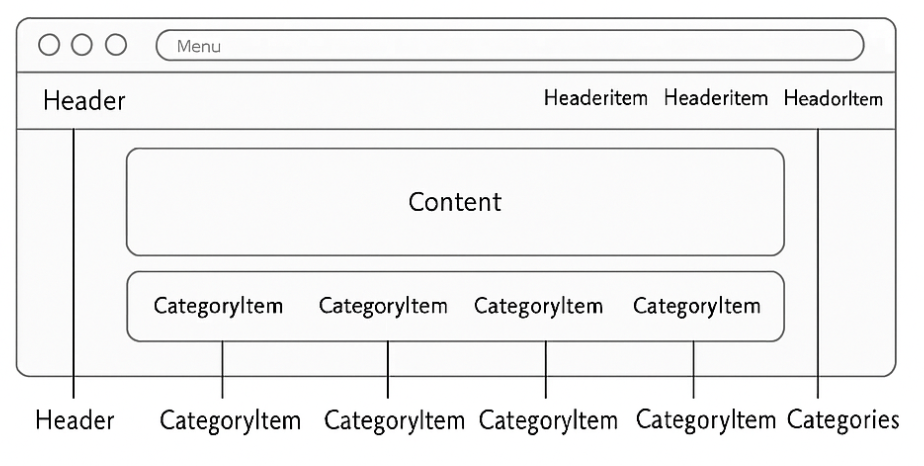
\includegraphics[width=0.85\textwidth]{REACT_NATIVE/images/A_text-based_digital_educational_graphic_offers_a_.png.png}
  \caption{Exemplo visual de componentização de um site com cabeçalho, categorias e conteúdo}
  \label{fig:componentizacao}
\end{figure}

Na Figura~\ref{fig:componentizacao}, temos uma interface simples de um site que foi dividida em componentes:

\begin{itemize}
  \item Um componente \texttt{Header}, responsável pela parte superior do site.
  \item Dentro do \texttt{Header}, componentes \texttt{HeaderItem} para cada item do menu.
  \item Um componente \texttt{Categorias}, que agrupa diversos componentes \texttt{CategoriaItem}.
  \item Outros elementos como a logo, barra de busca e sacola de compras também podem ser componentes reutilizáveis.
\end{itemize}

Essa flexibilidade é uma das maiores vantagens do React. Não existe uma única forma correta de dividir os componentes — essa decisão depende do projeto, da equipe e do contexto. O importante é que cada componente seja uma unidade funcional, reutilizável e de responsabilidade única.

\subsection*{Virtual DOM: performance com eficiência}

Outra inovação poderosa do React é o uso do \textit{Virtual DOM} — uma representação leve da estrutura de elementos da interface mantida em memória. Sempre que um componente sofre uma alteração (por exemplo, o usuário digita em um campo de texto), o React atualiza o Virtual DOM e compara com a versão anterior. Apenas as mudanças reais são aplicadas ao DOM do navegador.

Esse processo é conhecido como \textit{reconciliação} e é o que torna as aplicações React extremamente rápidas, pois evita recarregamentos desnecessários.

\subsection*{E o React Native?}

O React Native segue a mesma filosofia do React para web: dividir a interface em componentes reutilizáveis. A principal diferença está no ambiente de execução. Enquanto o React web manipula o DOM do navegador, o React Native se comunica com APIs nativas do sistema operacional por meio de uma ponte chamada \textit{Bridge}.

Essa ponte permite que o código JavaScript interaja diretamente com componentes nativos escritos em Java (Android) ou Swift/Objective-C (iOS). Com isso, conseguimos desenvolver aplicações verdadeiramente nativas, mas com a simplicidade e poder do React.



\section*{Código-fonte}
Código-fonte deste capítulo encontra-se em \href{https://github.com/hrausch/academico-react-native/tree/aula-04}{https://github.com/hrausch/academico-react-native/tree/aula-04} .



\chapter{Componentes em React}

\section{O que são componentes?}

\section{O que são componentes em React?}

Os componentes são a base da construção de interfaces no React. Eles permitem que uma aplicação seja dividida em pequenas partes isoladas, reutilizáveis e independentes, facilitando tanto o desenvolvimento quanto a manutenção do código.

Conceitualmente, um componente React é uma função (ou uma classe) JavaScript que recebe entradas chamadas \textit{props} e retorna elementos React — estruturas escritas em JSX que definem o que será exibido na tela.

Ao adotar a abordagem baseada em componentes, o React possibilita que cada parte da interface de usuário seja tratada de forma individual, com responsabilidades bem definidas. Essa divisão modular torna o desenvolvimento mais organizado, promove o reuso de código e facilita o trabalho em equipe.

Segundo a documentação oficial \cite{reactDocsComponents}, os componentes permitem "dividir a interface de usuário em partes independentes, reutilizáveis e pensar em cada parte isoladamente".

Essa filosofia se aplica tanto ao React para web quanto ao React Native, permitindo o uso de uma mesma lógica de construção de interfaces em múltiplas plataformas.


\section{Componentes funcionais}

Atualmente, os \textbf{componentes funcionais} são a forma mais recomendada de criar componentes em React. Eles são criados com funções JavaScript padrão e retornam JSX (uma extensão de sintaxe que parece HTML). Veja um exemplo simples:

\begin{lstlisting}[language=JavaScript, caption={Componente funcional PrimeiroComponente.js}]
import React from 'react';
import { Text, View } from 'react-native';

export default function PrimeiroComponente() {
  return (
    <View>
      <Text>Olá</Text>
      <Text>Mundo!</Text>
    </View>
  );
}
\end{lstlisting}

No exemplo acima, criamos um componente chamado \texttt{PrimeiroComponente} que retorna uma \texttt{<View>} contendo dois textos. No React Native, o \texttt{<View>} funciona como uma \texttt{<div>} no HTML, e o \texttt{<Text>} é equivalente a um \texttt{<p>} ou qualquer elemento de texto.

\subsection*{Atenção ao retorno dos componentes}

No React, um componente deve retornar apenas um elemento JSX. Portanto, se quisermos retornar dois ou mais elementos “irmãos”, devemos agrupá-los dentro de uma tag como \texttt{<View>} ou utilizar um fragmento \texttt{<></>}. Caso contrário, o React emitirá o erro:

\textit{Adjacent JSX elements must be wrapped in an enclosing tag.}

\section{Organizando os componentes}

Seguindo boas práticas do mercado, é comum criar uma pasta chamada \texttt{components} na raiz do projeto. Dentro dessa pasta, todos os componentes são criados e, conforme o projeto cresce, ela pode ser subdividida em categorias.

\textbf{Exemplo de estrutura de projeto:}

\begin{lstlisting}[language=bash]
meu-app/
├── App.js
├── components/
│   └── PrimeiroComponente.js
\end{lstlisting}

\section{Importando e utilizando componentes}

Uma vez criado o componente, podemos importá-lo e utilizá-lo em outros arquivos, como no \texttt{App.js}:

\begin{lstlisting}[language=JavaScript, caption={Importando e utilizando um componente personalizado}]
import React from 'react';
import { StyleSheet, Text, View } from 'react-native';
import PrimeiroComponente from './components/PrimeiroComponente';

export default function App() {
  return (
    <View style={styles.container}>
      <Text>Bem-vindo ao React Native!</Text>
      <PrimeiroComponente />
    </View>
  );
}

const styles = StyleSheet.create({
  container: {
    flex: 1,
    backgroundColor: '#fff',
    alignItems: 'center',
    justifyContent: 'center',
  },
});
\end{lstlisting}

O arquivo \texttt{PrimeiroComponente.js} conterá o seguinte:

\begin{lstlisting}[language=JavaScript, caption={Conteúdo de PrimeiroComponente.js}]
import React from 'react';
import { Text, View } from 'react-native';

export default function PrimeiroComponente() {
  return (
    <View>
      <Text>Olá</Text>
      <Text>Mundo!</Text>
    </View>
  );
}
\end{lstlisting}

\subsection*{Renomeando o componente na importação}

O nome da tag JSX usada para renderizar o componente é definido de acordo com o nome da variável usada na importação, e não necessariamente pelo nome da função exportada. Veja o exemplo abaixo:

\begin{lstlisting}[language=JavaScript, caption={Importando com outro nome}]
import TioPatinhas from './components/PrimeiroComponente';

export default function App() {
  return (
    <View>
      <TioPatinhas />
    </View>
  );
}
\end{lstlisting}

Neste caso, mesmo que o nome da função exportada dentro do arquivo seja \texttt{PrimeiroComponente}, o componente será renderizado como \texttt{<TioPatinhas />} pois é o nome dado na importação.

\section{Propriedades \texttt{props}}

As propriedades, conhecidas como \texttt{props}, são um mecanismo essencial no React para a comunicação entre componentes. Elas permitem passar informações de um componente pai para um componente filho, tornando os componentes mais flexíveis, reutilizáveis e dinâmicos \cite{rocketseatComponents}.

Conceitualmente, \texttt{props} são objetos que carregam pares de chave e valor — os atributos declarados na chamada do componente.

\subsection*{Exemplo básico}

Abaixo vemos um componente que recebe uma \texttt{prop} chamada \texttt{nome} e a exibe na tela:

\begin{lstlisting}[language=JavaScript, caption={Componente recebendo props}]
export const Saudacao = (props) => {
    return (
      <Text>Olá, {props.nome}!</Text>
    );
  };

export function SaudacaoCompleta(props) {
    return (
      <Text>
        Olá, {props.nome}! Você tem {props.idade} anos.
      </Text>
    );
  }
\end{lstlisting}

E sua utilização dentro de outro componente:

\begin{lstlisting}[language=JavaScript]
import { Saudacao, SaudacaoCompleta} from './components/PrimeiroComponente';

export default function App() {
  return (
    <View style={styles.container}>
      <Text>Olá, Mundo!</Text>
      <Saudacao nome="João" />
      <SaudacaoCompleta nome="Maria" idade={30} />
      <StatusBar style="auto" />
    </View>
  );
}
\end{lstlisting}

Nesse exemplo, o valor "Leitor" é passado como atributo do componente e acessado internamente via \texttt{props.nome}.

\subsection*{Importando componentes com e sem chaves}

Aqui está um ponto importante: a forma como o componente é exportado afeta diretamente como ele será importado em outro arquivo.

\begin{itemize}
  \item Para o \texttt{export default}, usamos \textbf{sem chaves}:
  \begin{lstlisting}[language=JavaScript]
import PrimeiroComponente from './components/PrimeiroComponente';
  \end{lstlisting}

  \item Para \texttt{export} nomeado, usamos \textbf{com chaves}:
  \begin{lstlisting}[language=JavaScript]
import {PrimeiroComponente, Saudacao, SaudacaoCompleta} from './components/PrimeiroComponente';
  \end{lstlisting}
\end{itemize}

Se você tentar importar um componente nomeado sem usar chaves, receberá um erro dizendo que o módulo não contém a exportação padrão.

\subsection*{Por que usamos \texttt{\{ \}} para passar números em props?}

Em React (JSX), quando passamos um valor para uma propriedade (prop), precisamos usar chaves \texttt{\{\}} sempre que o valor for uma expressão JavaScript — como um número, booleano, variável ou função.

Por exemplo, veja a diferença entre:

\begin{lstlisting}[language=JavaScript]
<SaudacaoCompleta nome="Maria" idade={30} /> // correto: número
<SaudacaoCompleta nome="Maria" idade="30" /> // também funciona, mas é string
\end{lstlisting}

No primeiro caso, \texttt{30} é um número. No segundo, \texttt{"30"} é uma string. Se quisermos realizar cálculos com esse valor dentro do componente, é importante que ele seja passado como número (usando \texttt{\{30\}}).

\subsubsection*{Resumo de como passar diferentes tipos de dados em props}

\begin{center}
\begin{tabular}{|l|l|l|}
\hline
\textbf{Tipo de valor} & \textbf{Como passar no JSX} & \textbf{Exemplo} \\
\hline
Texto (string)   & Entre aspas duplas              & \texttt{nome="Maria"} \\
Número           & Entre chaves                    & \texttt{idade=\{30\}} \\
Booleano         & Entre chaves                    & \texttt{ativo=\{true\}} \\
Variável         & Entre chaves                    & \texttt{idade=\{minhaIdade\}} \\
Expressão        & Entre chaves                    & \texttt{total=\{qtd * preco\}} \\
Função           & Entre chaves                    & \texttt{onClick=\{handleClick\}} \\
Objeto ou Array  & Entre chaves com estrutura      & \texttt{dados=\{\{nome: "Maria"\}\}} \\
\hline
\end{tabular}
\end{center}

Sempre que o valor passado for algo que o JavaScript possa avaliar (em vez de texto literal), use as chaves \texttt{\{\}}. Isso garante que o componente receba o dado corretamente tipado e funcional.



\subsection*{Props como children}

Todo componente React também possui uma propriedade especial chamada \texttt{children}, que representa tudo o que estiver entre a abertura e o fechamento da tag do componente.

\begin{lstlisting}[language=JavaScript, caption={Uso de props.children}]
const Card = (props) => {
  return (
    <View>
      {props.children}
    </View>
  );
};

const App = () => {
  return (
    <Card>
      <Text>Conteúdo dentro do Card!</Text>
    </Card>
  );
};
\end{lstlisting}

Isso permite criar estruturas reutilizáveis e aninhadas com flexibilidade.

\subsection*{Convenções e boas práticas}

\begin{itemize}
  \item Nomes de componentes devem começar com letra maiúscula.
  \item Props podem ter qualquer nome — você define.
  \item As tags podem ser escritas como \texttt{<Componente />} ou \texttt{<Componente></Componente>}.
\end{itemize}

Para mais informações, consulte a documentação oficial sobre \textit{props} em: \url{https://pt-br.legacy.reactjs.org/docs/components-and-props.html}

\section{Composição de Componentes}

Uma das grandes forças do React está na sua capacidade de composição. Isso significa que um componente pode conter outros componentes dentro de si, como se fosse montar uma interface com peças de LEGO.

Esse conceito nos permite dividir aplicações complexas em partes menores, facilitando a manutenção e a reutilização do código \cite{devtoComponentes, reactDocsComponents}.

\subsection*{Exemplo de composição}

Imagine uma tela inicial composta por cabeçalho, menu, carrossel, conteúdo e rodapé. Podemos criar um componente \texttt{Home} que agrupa todos esses elementos:

\begin{lstlisting}[language=JavaScript, caption={Composição de componentes}]
const Home = () => {
  return (
    <>
      <Header />
      <NavBar />
      <Carrousel />
      <Conteudo />
      <Footer />
    </>
  );
};

export default Home;
\end{lstlisting}

Cada componente acima pode ser desenvolvido de forma independente, testado isoladamente e reutilizado em outras partes do projeto.


\section{Múltiplos componentes por arquivo}

No React, é perfeitamente possível criar mais de um componente dentro de um mesmo arquivo \texttt{.js}. Essa prática é recomendada quando:

\begin{itemize}
  \item Os componentes são pequenos e utilizados apenas dentro daquele contexto.
  \item Há uma forte relação entre eles (por exemplo, \texttt{Card}, \texttt{CardHeader}, \texttt{CardBody}).
  \item Você quer reduzir a fragmentação do projeto em arquivos muito pequenos.
\end{itemize}

Para componentes maiores ou reutilizáveis entre várias telas, o ideal é separá-los em arquivos próprios, respeitando o princípio da responsabilidade única.


Por exemplo, podemos ter um arquivo chamado \texttt{Layout.js} que contém os componentes \texttt{Header}, \texttt{Footer} e um componente principal \texttt{Main}:

\begin{lstlisting}[language=JavaScript, caption={Vários componentes no mesmo arquivo}]
import React from 'react';
import { View, Text } from 'react-native';

export const Header = () => (
  <View><Text>Header</Text></View>
);

export const Footer = () => (
  <View><Text>Footer</Text></View>
);

const Main = () => (
  <View>
    <Header />
    <Text>Conteúdo Principal</Text>
    <Footer />
  </View>
);

export default Main;
\end{lstlisting}

Neste exemplo, temos:

\begin{itemize}
  \item Um \textbf{componente principal} chamado \texttt{Main}, que está sendo exportado como \texttt{default}.
  \item Dois \textbf{componentes auxiliares} \texttt{Header} e \texttt{Footer}, \textit{named exported}.
\end{itemize}

\subsection*{Importando componentes com e sem chaves (again)}

Aqui está um ponto importante: a forma como o componente é exportado afeta diretamente como ele será importado em outro arquivo.

\begin{itemize}
  \item Para o \texttt{export default}, usamos \textbf{sem chaves}:
  \begin{lstlisting}[language=JavaScript]
import Main from './Layout';
  \end{lstlisting}

  \item Para \texttt{named export}, usamos \textbf{com chaves}:
  \begin{lstlisting}[language=JavaScript]
import { Header, Footer } from './Layout';
  \end{lstlisting}
\end{itemize}

Se você tentar importar um componente nomeado sem usar chaves, receberá um erro dizendo que o módulo não contém a exportação padrão\cite{rocketseatExports}.


\section{Documentação oficial de componentes}

Todos os componentes padrão do React DOM estão documentados em:

\begin{quote}
\url{https://react.dev/reference/react-dom/components}
\end{quote}

Para o React Native, a lista de componentes e suas propriedades pode ser consultada em:

\begin{quote}
\url{https://reactnative.dev/docs/components-and-apis}
\end{quote}


\section*{Código-fonte}
Código-fonte deste capítulo encontra-se em \href{https://github.com/hrausch/academico-react-native/tree/aula-05}{https://github.com/hrausch/academico-react-native/tree/aula-05} .

\section*{Atividade Prática – Criando uma Mini Página com React Native}

\subsection*{Objetivo}
Aplicar os conceitos de componentes funcionais, props, composição e diferentes formas de exportação (\texttt{default} e \texttt{named}) aprendidos nas aulas anteriores.

\subsection*{Descrição da atividade}

Crie um aplicativo React Native utilizando Expo que represente uma pequena página de perfil. O aplicativo deverá ser estruturado com os seguintes componentes:

\begin{enumerate}
  \item \textbf{Header} (componente nomeado): Exibe o título “Bem-vindo ao App de Perfil”.
  
  \item \textbf{UserInfo} (componente nomeado): Recebe e exibe as seguintes \texttt{props}:
  \begin{itemize}
    \item \texttt{nome}
    \item \texttt{idade}
    \item \texttt{email}
  \end{itemize}
  
  \item \textbf{MensagemPersonalizada} (componente nomeado): Recebe como prop o nome do usuário e exibe a seguinte mensagem: \texttt{Olá, [nome]! Que bom ver você por aqui.}
  
  \item \textbf{Footer} (componente nomeado): Exibe o rodapé com o ano atual.
  
  \item \textbf{App} (componente com \texttt{export default}): Componente principal que importa e renderiza os demais componentes.
\end{enumerate}



\vspace{0.5cm}
\noindent
\textbf{Exemplo de estrutura esperada no retorno do componente App:}

\begin{lstlisting}[language=JavaScript]
<Header />
<UserInfo nome="Ana" idade={25} email="ana@email.com" />
<MensagemPersonalizada nome="Ana" />
<Footer />
\end{lstlisting}

\vspace{0.5cm}

\subsection*{Critérios de avaliação}

\begin{itemize}
  \item Uso correto de componentes funcionais
  \item Utilização adequada de \texttt{props}
  \item Composição e reutilização de componentes
  \item Uso de \texttt{export default} e \texttt{named exports}
  \item Organização e clareza do código
\end{itemize}





%https://blog.geekhunter.com.br/criando-componentes-react-componentes-de-classe-e-funcional-sem-estado/
\appendix
\chapter{Sequência de Comandos para Criar e Executar Aplicações React com Expo}

A tabela a seguir apresenta a sequência de comandos necessária para instalar, criar e executar um aplicativo React utilizando Expo, tanto no ambiente local quanto de forma dockerizada.

\begin{longtable}{|p{5cm}|p{9cm}|}
\hline
\textbf{Etapa} & \textbf{Comando} \\
\hline
\multicolumn{2}{|c|}{\textbf{Instalação e uso sem Docker}} \\
\hline
Instalar Expo CLI & 
\texttt{npm install -g expo-cli} \\
\hline
Criar novo aplicativo & 
\texttt{expo init nome-do-app} \newline
Selecionar o template \texttt{blank} \\
\hline
Entrar na pasta do projeto & 
\texttt{cd nome-do-app} \\
\hline
Instalar suporte Web (obrigatório) & 
\texttt{npx expo install react-dom react-native-web @expo/metro-runtime} \\
\hline
Rodar a aplicação & 
\texttt{npm start}  \\
\hline
\hline
\end{longtable}



\bibliographystyle{plain} % ou abnt, ieee, apalike, etc.
\bibliography{referencias}



\end{document}
